\documentclass[10pt,a4paper,twoside]{article}
\usepackage[utf8]{inputenc}
\usepackage[francais]{babel}
\usepackage[T1]{fontenc}
\usepackage{graphicx}

\usepackage{geometry}
\geometry{hmargin=3cm,vmargin=4cm}

\author{Florant Clément - Lezaud Victor - Zamora Benjamin}
\title{TP POO 2 - Pointeurs et Polymorphisme}
\begin{document}

\maketitle
\renewcommand{\contentsname}{Sommaire}
\tableofcontents

\newpage
\section{Hiérarchie de classe}
\subsection{Diagramme}
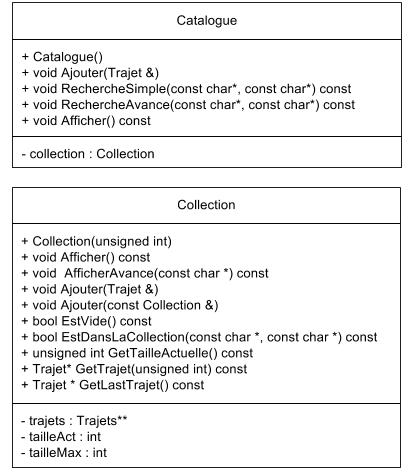
\includegraphics[scale=0.6]{classe2.jpg} \\
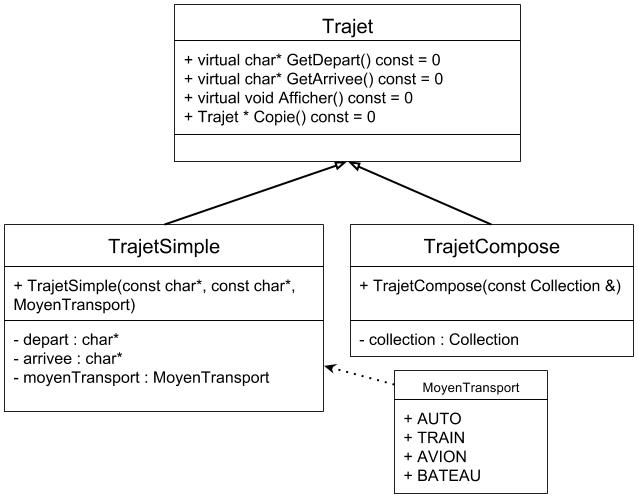
\includegraphics[scale=0.5]{classe1.jpg} 

\subsection{Justification}
\subsubsection{Trajet - TrajetSimple - TrajetCompose}
TrajetSimple et TrajetCompose sont des sortes de Trajet, les classes héritent donc publiquement de Trajet. La classe abstraite Trajet ne sert qu'à définir une interface, toutes ses méthode sonts virtuelles pures et elle ne possède pas d'attributs. C'est pour cela que les classes TrajetSimple et TrajetCompose redéfinissent ces méthodes en accord avec les attributs qui leurs sont propres

\subsubsection{Catalogue}
Le Catalogue est l'objet principal du programme, ses méthodes définissent les services proposés par le programme (Ajouter, RechercheSimple et RechercheAvance).

\subsubsection{Collection}
La Collection sert de conteneur pour les Trajet de Catalogue et TrajetCompose. Elle est ici implémentée avec un tableau dynamique de pointeur de trajet. Comme on utilise la Collection à chaque fois que l'on veut stocker plusieurs Trajet elle doit offrir beaucoup de services d'où ce grand nombre méthodes.\\
Il est très important que la Colletion stocke des pointeurs sur Trajets afin de pouvoir user du polymorphisme ce qui est nécessaire pour ce programme.

\newpage
\section{Spécification}
\subsection{Classe Trajet}
\subsubsection{Présentation}
La classe Trajet symbolise un trajet quelconque. C'est une classe abstraite.

\subsubsection{Attributs}
La classe n'a pas d'attributs.

\subsubsection{Méthodes}
\begin{itemize}
\item La construction sera interdite (Constructeurs déclarés protected).
\item \verb$virtual char * GetDepart(void) const = 0$ : renvoie le nom de la ville de départ. La méthode est virtuelle pure.
\item \verb$virtual char * GetArrivee(void) const = 0$ : renvoie le nom de la ville d'arrivée. La méthode est virtuelle pure.
\item \verb$virtual Trajet * Copie(void) const = 0$ : Renvoie un pointeur sur une copie de l'objet allouée dynamiquement.
\item \verb$virtual void Afficher(void) const = 0$ : permet d'afficher en console les informations liées à l'objet. La méthode est virtuelle pure.
\end{itemize}


\subsection{Classe TrajetSimple}
\subsubsection{Présentation}
La classe TrajetSimple symbolise un trajet direct d'une ville de départ à une ville d'arrivée en utilisant un moyen de transport précis. Un TrajetSimple est une sorte de Trajet, cette classe hérite donc publiquement de la classe Trajet.

\subsubsection{Enumeration MoyenTransport}
\paragraph{Présentation :} 
La classe TrajetSimple possède une énumération MoyenTransport qui décrit les différents moyens de transport disponible.
\paragraph{Valeur :} 
L'énumération peut prendre les valeurs suivantes:
\begin{itemize}
\item AUTO
\item BATEAU
\item AVION
\item TRAIN
\end{itemize}
\paragraph{Fonction associée :} 
L'affichage des TrajetSimple nécessite une fonction qui affiche une chaîne de caractère décrivant le moyen de transport avec la signature suivante, et qui affiche simplement le nom du MoyenTransport sans espaces ni retour à la ligne :\\
\verb=void AfficherMoyenTransport(MoyenTransport moyenTransport)=

\subsubsection{Attributs}
\begin{itemize}
\item \verb=MoyenTransport moyenTransport= : variable de l'énumération MoyenTransport qui stocke le moyen de transport utilisé par le trajet
\item \verb=depart= : variable stockant la ville de départ
\item \verb=arrivee= : variable stockant la ville d'arrivée
\end{itemize}
\subsubsection{Méthodes}
\begin{itemize}
\item Le constructeur par défaut sera interdit (Constructeur par défaut déclaré protected).
\item \verb=TrajetSimple(const char* villeDepart, const char* =\\
\verb=villeArrivee, Vehicule transport)= : Constructeur de la classe
\item \verb=TrajetSimple(const TrajetSimple & copie)= : Constructeur de copie de la classe

\end{itemize}

\subsection{Classe TrajetCompose}
\subsubsection{Présentation}
La classe TrajetCompose symbolise un trajet ayant des étapes. Il contient donc une Collection de Trajet. Un TrajetCompose est une sorte de Trajet, cette classe hérite donc publiquement de la classe Trajet.
\subsubsection{Attributs}
\begin{itemize}
\item \verb=Collection collection=: contient la liste des Trajets qui compose ce TrajetCompose
\end{itemize}
\subsubsection{Méthodes}
\begin{itemize}
\item Le constructeur par défaut sera interdit (Constructeur par défaut déclaré protected).
\item \verb$TrajetCompose(const Collection & collec)$ : Constructeur de la classe
\item \verb=TrajetCompose(const TrajetCompose & copie)= : Constructeur de copie de la classe
\end{itemize}

\subsection{Catalogue}
\subsubsection{Présentation}
La classe Catalogue symbolise un ensemble de trajet, dans lequel on peut rechercher l'ensemble des trajets permettant d'aller d'une ville A à une ville B (avec ou sans combinaison de trajet).
\subsubsection{Attributs}
\begin{itemize}
\item \verb=Collection collection= : contient l'ensemble des trajets présents dans le catalogue
\end{itemize}
\subsubsection{Méthodes}
\begin{itemize}
\item \verb$Catalogue()$ : Constructeur de la classe
\item \verb=void Ajouter(Trajet & unTrajet)= : Permet d'ajouter un trajet au catalogue
\item \verb=void RechercheSimple(const char* villeDepart,=  \\
\verb=const char* villeArrivee) const=: Recherche et affiche l'ensemble des trajets permettant d'aller de villeDepart à villeArrivee sans combinaisons
\item \verb=void RechercheAvance(const char* villeDepart,= \\
\verb=const char* villeArrivee) const=: Recherche et affiche l'ensemble des trajets permettant d'aller de villeDepart à villeArrivee avec combinaisons. On ne réalisera pas deux fois le même trajet dans une solution (même ville de départ, même ville d'arrivée)
\item \verb=void Afficher(void) const= : permet d'afficher en console les informations liées à l'objet. 
\end{itemize}

\subsection{Classe Collection}
\subsubsection{Présentation}
La classe collection contient une liste ordonnée de Trajet*. Aujourd'hui nous l'implémentons avec un tableau dynamique.

\subsubsection{Attributs}
\begin{itemize}
\item \verb=Trajet** tab= : contient l'ensemble des trajets présents dans la collection
\item \verb=int tailleAct= : contient le nombre de trajet présents dans la collection
\item \verb=int tailleMax= : contient le nombre de case allouées en mémoire pour la collection
\end{itemize}

\subsubsection{Méthodes}
\begin{itemize}
\item \verb$Collection(unsigned int taille = 1)$= : Constructeur de la classe alloue un tableau de la taille donnée en paramètre. Sert aussi de constructeur par défaut.
\item \verb=Collection(const Collection & collection)= : Constructeur de copie de la classe
\item \verb=void Ajouter(Trajet & trajet)= : Ajoute un trajet à la collection. Le trajet est ajouté en fin de tableau.
\item \verb=void Ajouter(const Collection & autre)= : Ajoute à la collection l'ensemble des trajet de l'autre collection
\item \verb=Trajet * GetTrajet(unsigned int index) const= : Renvoie le trajet stocké à la position donnée en paramètre.
\item \verb=Trajet * GetLastTrajet(void) const= : Renvoie un pointeur vers le dernier trajet
\item \verb=unsigned int GetTailleActuelle(void) const= : Renvoie la taille actuelle de la collection
\item \verb=bool EstVide() const= : Renvoie true si le catalogue est vide
\item \verb=bool EstDansLaCollection(const char* depart, const char* arrivee) const= : Renvoie true si il existe un trajet allant de depart a arrivee dans la collection
\item \verb=void Afficher() const= : Affiche la liste des trajets présents dans la collection
\item \verb=void AfficherAvance(const char * arrivee) const= : Permet d'afficher la collection comme un résultat de recherche avancée
\end{itemize}

\subsection{Programme Principal}
\subsubsection{Présentation}
Le programme principal crée un catalogue puis il affiche en boucle un menu offrant à l'utilisateur les options suivantes :
\begin{itemize}
\item Ajouter un trajet au catalogue.
\item Effectuer une recherche de trajet (recherche simple)
\item Effectuer une recherche de trajet (recherche avancée)
\item Fermer le programme 
\end{itemize}

\subsubsection{Fonctionnement}
\paragraph{Menu Principal :} Le choix de l'utilisateur sera fait en entrant le numéro associé à l'option qu'il souhaite. Le programme devra donc effectuer la requête de l'utilisateur avant de ré-afficher le menu principal.
\paragraph{Ajout de trajet :} Pour l'ajout de trajet, l'utilisateur doit d'abord choisir entre un trajet direct ou un trajet avec étape. 
\begin{itemize}
\item Trajet direct : Pour l'ajout d'un trajet direct l'utilisateur n'a qu'à entrer la ville de départ, la ville d'arrivée et le moyen de transport.
\item Trajet avec étape : Pour un trajet avec étape on réalise l'ajout d'un trajet direct puis on demande si l'utilisateur souhaite ajouter une autre étape. On recommence l'opération jusqu'à ce que l'utilisateur ne souhaite plus ajouter d'étape.
\end{itemize}

\paragraph{Recherche de Trajet :} L'utilisateur rentre la ville de départ puis la ville d'arrivée. Le programme affiche l'ensemble des trajets répondants à la requête. Il y a deux versions de la recherche : simple et avancée.
\paragraph{Fermer le programme :} Le programme sors de la boucle, libère toute la mémoire allouée et se ferme.

\subsubsection{Affichage}
\paragraph{Menu Principal :}
\begin{verbatim}
----------- Menu Principal -----------
1. Ajouter un trajet au catalogue
2. Effectuer une recherche de trajet (recherche simple)
3. Effectuer une recherche de trajet (recherche avancée)
0. Sortir du programme
---Votre choix : <entrée au clavier>
\end{verbatim}

\paragraph{Ajout de trajet}
\begin{verbatim}
----------- Ajout de Trajet -----------
Ville de départ : <entrée au clavier>
Ville d'arrivée : <entrée au clavier>
Moyen de Transport:
1. Auto
2. Bateau
3. Train
4. Avion
---Votre choix: <entrée au clavier>
--- Voulez-cous ajoutez une étape ? (O/N)
--- Votre choix : <entrée au clavier>
----------- Fin Ajout de Trajet -----------
\end{verbatim}

\paragraph{Recherche de Trajet :}
\begin{verbatim}
----------- Début Recherche de Trajet -----------
Ville de départ : <entrée au clavier>
Ville d'arrivée : <entrée au clavier>
---------- Résultat de la recherche  ----------
Nombre de réponse : <nb réponse>
-------Trajet numéro <i> :
Affichage trajet i

---------- Fin Recherche de Trajet ----------
\end{verbatim}


\newpage
\section{Structure de données}
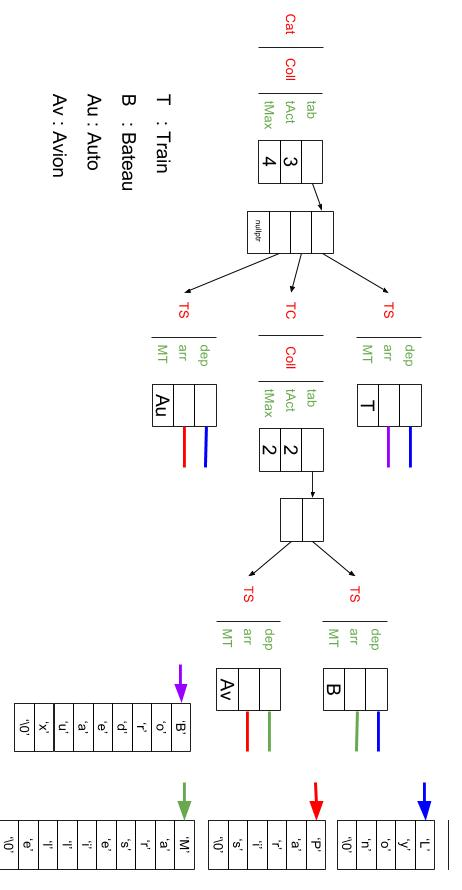
\includegraphics[scale=0.7]{dessin_memoire_TP_POO_2.jpg} 
%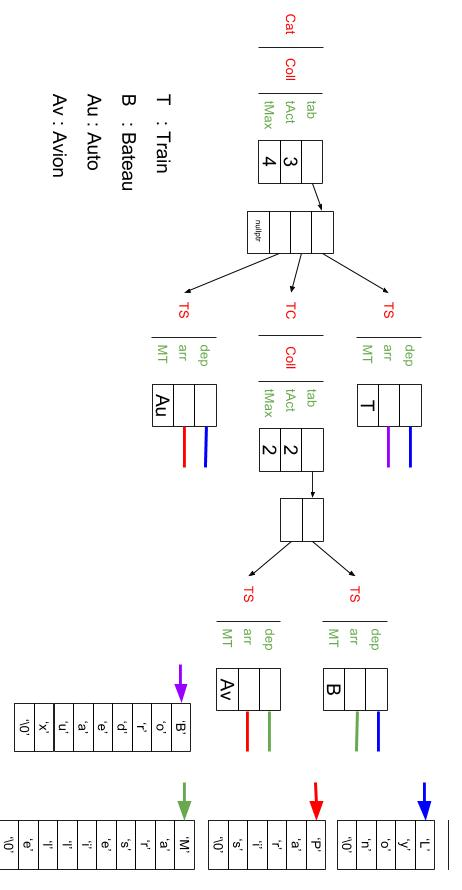
\includegraphics[scale=0.5]{dessin_memoire_TP_POO_2.jpg} 

\newpage
\section{Problèmes rencontrés}
\subsection{Gestion de la mémoire}
\subsubsection{Présentation du problème}
Lorsque nous avons commencé à implémenter la construction d'un TrajetCompose à l'aide d'une collection nous avons eu des problèmes de gestion de la mémoire. Le constructeur par copie de la collection réalisait une copie des valeurs des pointeurs contenus dans la collection. De cette manière la destruction de la collection passée en paramètre ou celle du TrajetCompose libérait la zone de mémoire utilisée par l'autre. L'exécution menait donc à une segmentation fault.

\subsubsection{Solutions possibles}
Nous avons réfléchis à deux solutions possibles:
\paragraph{Attribut pointeur sur Collection :} Une façon de régler le problème serait de modifier le type de l'attribut de la classe TrajetCompose en pointeur sur Collection et passer au constructeur un pointeur sur Collection et non plus une référence. Ainsi la Collection ne serait plus dupliquée
\paragraph{Copie en profondeur de la Collection :} Une autre solution est de copier en profondeur la Collection. Il s'agit donc de ne plus copier l'adresse contenus dans les pointeurs mais bien de dupliquer les objets pointés par les pointeurs. Ainsi la destruction d'une Collection n'aura plus aucun effet sur les objets de l'autre.
\paragraph{Solution choisie :} Nous avons décidé d'implémenter la deuxième solution car elle nous permettait de conserver l'ensemble de notre code réaliser jusque là (les méthodes d'ajout de trajet par l'utilisateur, le constructeur de copie de TrajetCompose, etc...).

\subsubsection{Difficulté de la solution}
\paragraph{Description de la difficulté :} La complexité de cette solution réside dans l'utilisation du polymorphisme par l'objet Collection lequel possède des pointeurs sur Trajet qui pointent sur des TrajetSimple et des TrajetCompose. Or nous ne devons pas perdre d'information.

\paragraph{Solution :} La solution à ce problème passe par une liaison dynamique grâce a mot clé virtual. En effet on doit réaliser un traitement différent en fonction de la classe de l'objet, laquelle est inconnue avant l'exécution. On déclare donc une méthode virtuelle pure dans Trajet, nommée Copie, puis on la définit dans TrajetSimple et TrajetCompose. La méthode Copie crée avec une allocation dynamique une copie de l'objet appelant la méthode et renvoie un pointeur vers le nouvel objet.

\subsection{Algorithmie}

\subsubsection{Présentation du problème}
\paragraph{Méthode concernée :} La recherche avancée est de loin la partie la complexe du programme algorithmiquement. Nous n'avons eu aucun problème de structures de données car la classe collection était parfaitement utilisable pour réaliser cette algorithme. Le problème est plutôt lié à l'aspect récursif de la méthode.
\paragraph{Description du problème :} En effet lors d'un appel de la méthode récursive on trouve plusieurs objets Trajet qui permettent de continuer, donc cet appel va appeler plusieurs fois la méthode or nous avions une collection stockant les objets Trajet utilisés. La méthode ajoutait donc des objets Trajet en trop lorsque plusieurs Trajet partaient d'une même ville
\paragraph{Exemple de test :} Avec un catalogue contenant les trajets suivants :
\begin{itemize}
\item de A vers B
\item de B vers C
\item de B vers D
\item de C vers E
\item de D vers E
\end{itemize}
La recherche avencée de A vers E nous donnait :
\begin{itemize}
\item voyage 1:
\begin{itemize}
\item A vers B
\item B vers C
\item C vers E
\end{itemize}
\item voyage 2:
\begin{itemize}
\item A vers B
\item B vers C
\item B vers D
\item D vers E
\end{itemize}
\end{itemize}

\subsubsection{Algorithme solution}
\begin{verbatim}
void Catalogue::Recursion(const char* depart, const char* arrivee,
                          Collection TrajetsEmpruntes, Collection & result) const
{
    unsigned int i;
    for (i = 0; i < collection.GetTailleActuelle(); ++i)
    {
        Trajet* trajet = collection.GetTrajet(i);
        
        int compDepart = strcmp(depart, trajet->GetDepart());
        bool dejaEmprunte = TrajetsEmpruntes.EstDansLaCollection
                (trajet->GetDepart(), trajet->GetArrivee());
        
        // pour chaque trajet on teste si la ville de depart est bien depart
        // et on verifie que l'on ne l'ai pas deja emprunte
        
        if (compDepart == 0 && !dejaEmprunte)
        {
            Collection nvxTrajetsEmpruntes(TrajetsEmpruntes);
            nvxTrajetsEmpruntes.Ajouter(trajet->Copie());
            // On crée une copie de la Collection puis on ajoute le trajet courant
            
            int compArrivee = strcmp(arrivee, trajet->GetArrivee());
            
            if (compArrivee == 0)
            {
                // si on est arrive on ajoute les trajets a la collection result
                result.Ajouter(nvxTrajetsEmpruntes);
            }
            else
            {
                // sinon on appelle a nouveau la methode
                Recursion(trajet->GetArrivee(), arrivee,
                          nvxTrajetsEmpruntes,result);
            }
        }
    }
}
\end{verbatim}

La solution au problème exposée ci-dessus réside dans l'ajout d'une variable nvxTrajetsEmpruntes locale au bloc \verb$if(compDepart == 0 && !dejaEmprunte)$ ainsi on a bien une Collection différente pour chacun des Trajet.

\section{Piste d'amélioration}
\subsection{Optimisation}
Actuellement le programme réalise beaucoup de copie, d'allocation et de suppression notamment à cause de nombreux passage de Collection par valeur. Un piste d'amélioration serait de réduire ces copies et de remplacer des passages par valeurs par des passages par référence ou pointeur. Cela permettrait de rendre le programme plus rapide et moins gourmand en mémoire par moment.

\subsection{Stabilité}
Le programme est très peu robuste par rapport à ce que donne l'utilisateur en entrée : s'il ne respecte un format d'entrée spécifique le programme ne fonctionne plus. Avec les ajouts du cours POO2 sur les flux nous pourrions régler ce problème et rendre ainsi le programme plus stable.

\subsection{Ergonomie}
L'affichage en console n'est pas toujours très ergonomique et pas très esthétique. Ce point pourrait également être amélioré notamment grâce aux ajouts du cours POO2 sur les flux.

\newpage
\section{Code source}

\subsection{Module Trajet}
\subsubsection{Trajet.h}
\begin{verbatim}
//------- Interface de la classe <Trajet> (fichier Trajet.h) -------------
#if ! defined ( TRAJET_H )
#define TRAJET_H
//------------------------------------------------------------------------
// Rôle de la classe <Trajet>
//
//	La classe Trajet symbolise un trajet quelconque
//------------------------------------------------------------------------

class Trajet
{
//----------------------------------------------------------------- PUBLIC
    public:
//----------------------------------------------------- Méthodes publiques
        virtual char* GetDepart() const = 0;
        // renvoie le nom de la ville de depart
        
        virtual char* GetArrivee() const = 0;
        // renvoie le nom de la ville de depart
        
        virtual void Afficher() const = 0;
        // permet d’afficher en console les informations liées à l’objet.
        
        virtual Trajet* Copie() const = 0;
        // Renvoie un pointeur sur une copie distincte de ce trajet
        // Contrat :
        // Le pointeur retourné pointe sur un objet alloué dynamiquement
        // IL DOIT ETRE LIBERE PAR UN delete !!!
        
        virtual ~Trajet();
        // Destructeur de la classe

//-------------------------------------------------------------- PROTECTED
    protected:
//----------------------------------------------------- Méthodes protégées
        Trajet();
        // Constructeur de la classe
        
        Trajet(const Trajet & copie);
        // Constructeur de copie de la classe

};

#endif // TRAJET_H
\end{verbatim}


\newpage
\subsection{Trajet.cpp}
\begin{verbatim}
//------- Réalisation de la classe <Trajet> (fichier Trajet.cpp) ---------

//---------------------------------------------------------------- INCLUDE
//-------------------------------------------------------- Include système
using namespace std;
#include <iostream>

//------------------------------------------------------ Include personnel
#include "Trajet.h"
//-------------------------------------------- Constructeurs - destructeur

Trajet::Trajet ( )
{
#ifdef MAP
    cout << "Appel au constructeur de <Trajet>" << endl;
#endif
}

Trajet::Trajet (const Trajet & copie )
{
#ifdef MAP
    cout << "Appel au constructeur de copie de <Trajet>" << endl;
#endif
}

Trajet::~Trajet ( )
{
#ifdef MAP
    cout << "Appel au destructeur de <Trajet>" << endl;
#endif
}
\end{verbatim}


\newpage
\subsection{Module TrajetSimple}
\subsubsection{TrajetSimple.h}
\begin{verbatim}
//----- Interface de la classe <TrajetSimple.h> (fichier TrajetSimple.h) -----
#ifndef TRAJET_SIMPLE_H
#define TRAJET_SIMPLE_H

//-------------------------------------------------------- Interfaces utilisées
#include "Trajet.h"
//----------------------------------------------------------------------- Types
typedef enum {AUTO,AVION,BATEAU,TRAIN} MoyenTransport;
// L'enumeration recense les differents les moyen de transport utilisable pour
// les TrajetSimple

//-----------------------------------------------------------------------------
// Rôle de la classe <TrajetSimple>
// La classe TrajetSimple symbolise un trajet direct d'une ville depart a une
// ville arrivee a l'aide d'un moyen transport
// Un TrajetSimple est une sorte de Trajet
//-----------------------------------------------------------------------------

class TrajetSimple :public Trajet
{
	//------------------------------------------------------------------ PUBLIC
	public :
	//------------------------------------------------------ Méthodes publiques
	virtual char* GetDepart() const;
	// renvoie la valeur stockée dans l’attribut depart
	
	virtual char* GetArrivee() const;
	// renvoie la valeur stockée dans l’attribut arrivee
	
	virtual void Afficher() const;
	// permet d’afficher en console les informations liées à l’objet.
	// Les informations seront affichés ainsi :
	// TrajetSimple de <depart> à <arrivee>
	
	virtual Trajet* Copie() const;
	// Renvoie un pointeur sur une copie distincte de ce trajet
	// Contrat :
	// Le pointeur retourné pointe sur un objet alloué dynamiquement
	// IL DOIT ETRE LIBERE PAR UN delete !!!
	
	//--------------------------------------------- Constructeurs - Destructeur
	TrajetSimple(const char * villeDepart, const char * villeArrivee,
	MoyenTransport moyenTransport);
	// Constructeur de la classe
	
	TrajetSimple(const TrajetSimple & copie);
	// Constructeur de copie de la classe
	
	virtual ~TrajetSimple();
	// Destructeur de la classe
	
	//------------------------------------------------------------------- PRIVE
	protected:
	//------------------------------------------------------- Méthodes protégées
	TrajetSimple();
	// Constructeur par defaut de la classe
	
	//------------------------------------------------------- Attributes protégé
	char * depart;
	// ville de depart du Trajet
	
	char * arrivee;
	// ville d'arrivee du Trajet
	
	MoyenTransport vehicule;
	// moyen de transport utilise pendant le trajet
};

//----------------------------- Autres définitions dépendantes de <TrajetSimple>

void AfficherMT(MoyenTransport vehicule);
// Affiche le nom du moyen de transport

#endif // ! defined ( TRAJET_SIMPLE_H )
\end{verbatim}


\newpage
\subsubsection{TrajetSimple.cpp}
\begin{verbatim}
//-- Réalisation de la classe <TrajetSimple.cpp> (fichier TrajetSimple.cpp) ---

//--------------------------------------------------------------------- INCLUDE
//------------------------------------------------------------- include système
using namespace std;
#include <iostream>
#include <cstring>

//----------------------------------------------------------- include personnel
#include "TrajetSimple.h"

//------------------------------------------------------------------- constante
const char * nomTransport[] = {"voiture", "avion", "bateau", "train"};

//---------------------------------------------------------------------- PUBLIC
//---------------------------------------------------------- Méthodes publiques
char * TrajetSimple::GetDepart() const
{
    return depart;
}

char * TrajetSimple::GetArrivee() const
{
    return arrivee;
}

void TrajetSimple::Afficher() const
{
    cout << "Trajet direct de " << depart << " à " << arrivee << " en ";
    AfficherMT(vehicule);
    cout << endl;
}

Trajet* TrajetSimple::Copie() const
{
    Trajet* trajet = new TrajetSimple(*this);
    return trajet;
}

//------------------------------------------------- Constructeurs - destructeur

TrajetSimple::TrajetSimple(const char * villeDepart, const char * villeArrivee,
                     MoyenTransport moyenTransport) : vehicule(moyenTransport)
{
#ifdef MAP
cout<<"Appel au constructeur de <TrajetSimple>"<<endl;
#endif
    depart = new char[strlen(villeDepart)+1];
    arrivee = new char[strlen(villeArrivee)+1];
    
    strcpy(depart, villeDepart);
    strcpy(arrivee, villeArrivee);
    
}

TrajetSimple::TrajetSimple(const TrajetSimple & copie)
        : vehicule(copie.vehicule)
{
#ifdef MAP
cout<<"Appel au constructeur de copie de <TrajetSimple>"<<endl;
#endif
    depart = new char[strlen(copie.depart)+1];
    arrivee = new char[strlen(copie.arrivee)+1];
    
    strcpy(depart, copie.depart);
    strcpy(arrivee, copie.arrivee);
}

TrajetSimple::~TrajetSimple()
{
#ifdef MAP
cout << "Appel au destructeur de <TrajetSimple>" << endl;
#endif
    delete [] depart;
    delete [] arrivee;
}


void AfficherMT(MoyenTransport vehicule)
{
    cout << nomTransport[vehicule];
}
\end{verbatim}


\newpage
\subsection{Module TrajetCompose}
\subsubsection{TrajetCompose.h}
\begin{verbatim}
//----- Interface de la classe <TrajetCompose> (fichier TrajetCompose.h) ------
#ifndef TRAJET_COMPOSE_H
#define TRAJET_COMPOSE_H

//-------------------------------------------------------- Interfaces utilisées
#include "Collection.h"
#include "Trajet.h"

//-----------------------------------------------------------------------------
// Rôle de la classe <TrajetCompose>
// La classe TrajetCompose symbolise un trajet ayant des étapes. Il contient
// donc une liste ordonnée de Trajet. Un TrajetCompose est une sorte de Trajet,
// cette classe hérite donc publiquement de la classe Trajet.
//-----------------------------------------------------------------------------

class TrajetCompose :public Trajet
{
    //------------------------------------------------------------------ PUBLIC
    public :
    //------------------------------------------------------ Méthodes publiques
    virtual char* GetDepart() const;
    // renvoie la valeur stockée dans l’attribut depart
    
    virtual char* GetArrivee() const;
    // renvoie la valeur stockée dans l’attribut arrivee
    
    virtual void Afficher() const;
    // permet d’afficher en console les informations liées à l’objet.
    
    virtual Trajet* Copie() const;
    // Renvoie un pointeur sur une copie distincte de ce trajet
    // Contrat :
    // Le pointeur retourné pointe sur un objet alloué dynamiquement
    // IL DOIT ETRE LIBERE PAR UN delete !!!
    
    //--------------------------------------------- Constructeurs - Destructeur
    TrajetCompose(const Collection & collec);
    // Constructeur de la classe
    
    TrajetCompose(const TrajetCompose & copie);
    // Constructeur de copie de la classe
    
    virtual ~TrajetCompose();
    // Destructeur de la classe
    
    //------------------------------------------------------------------- PRIVE
    protected:
    //------------------------------------------------------ Attributes protégé
    Collection etapes;
    // Collection contenant la liste des etapes du TrajetCompose
};



#endif // ! defined ( TRAJET_COMPOSE_H )
\end{verbatim}


\newpage
\subsubsection{TrajetCompose.cpp}
\begin{verbatim}
//- Réalisation de la classe <TrajetCompose.cpp> (fichier TrajetCompose.cpp) --

//--------------------------------------------------------------------- INCLUDE
//------------------------------------------------------------- include système
using namespace std;
#include <iostream>

//----------------------------------------------------------- include personnel
#include "TrajetCompose.h"

//---------------------------------------------------------------------- PUBLIC
//---------------------------------------------------------- Méthodes publiques
char * TrajetCompose::GetDepart() const
{
    if(etapes.EstVide())
    {
        return nullptr;
    }
    return etapes.GetTrajet(0)->GetDepart();
}

char * TrajetCompose::GetArrivee() const
{
    if(etapes.EstVide())
    {
        return nullptr;
    }
    return etapes.GetLastTrajet()->GetArrivee();
}

void TrajetCompose::Afficher() const
{
    cout<<"Trajet composé des étapes suivantes :"<<endl;
    etapes.Afficher();
}

Trajet* TrajetCompose::Copie() const
{
    Trajet* trajet = new TrajetCompose(*this);
    return trajet;
}

//------------------------------------------------- Constructeurs - destructeur
TrajetCompose::TrajetCompose(const Collection & collec) : etapes(collec)
{
#ifdef MAP
    cout << "Appel au constructeur de <TrajetCompose>" << endl;
#endif
}

TrajetCompose::TrajetCompose(const TrajetCompose & copie)
        : etapes(copie.etapes)
{
#ifdef MAP
    cout << "Appel au constructeur de copie de <TrajetCompose>" << endl;
#endif
}

TrajetCompose::~TrajetCompose()
{
#ifdef MAP
    cout << "Appel au destructeur de <TrajetCompose>" << endl;
#endif
}
\end{verbatim}


\newpage
\subsection{Module Catalogue}
\subsubsection{Catalogue.h}
\begin{verbatim}
//------- Interface de la classe <Catalogue> (fichier Catalogue.h) ------------
#ifndef CATALOGUE_H
#define CATALOGUE_H

//-------------------------------------------------------- Interfaces utilisées
#include "Collection.h"

//------------------------------------------------------------------ Constantes


//------------------------------------------------------------------- Fonctions


// Effectue les operations recursives necessaires a la recherche avancee

//----------------------------------------------------------------------- Types


//-----------------------------------------------------------------------------
// Rôle de la classe <Catalogue>
// La classe Catalogue symbolise un ensemble de trajet, dans lequel on peut
// rechercher l’ensemble des trajets permettant d’aller d’une ville A à une
// ville B (avec ou sans combinaison de trajet).
//-----------------------------------------------------------------------------

class Catalogue
{
    //------------------------------------------------------------------ PUBLIC
    public :
    //------------------------------------------------------ Méthodes publiques
    void Ajouter(Trajet * unTrajet);
    // Permet d'ajouter un trajet au catalogue
    
    void Afficher() const;
    // Permet d'afficher les informations liées au catalogue
    
    Collection RechercheSimple(const char* depart, const char* arrivee) const;
    // Renvoie les trajets allant de depart à arrivee dans une collection
    
    Collection RechercheAvancee(const char* depart, const char* arrivee) const;
    // Renvoie les combinaisons de trajets allant de depart à arrivee dans une
    // collection sans reutiliser 2 fois le même trajet

    

    //--------------------------------------------- Constructeurs - Destructeur
    Catalogue();
    // Constructeur par défaut de la classe
    
    virtual ~Catalogue();
    // Destructeur de la classe
    
    //------------------------------------------------------------------- PRIVE
    protected:
    void Recursion(const char* depart, const char* arrivee,
                   Collection TrajetsEmpruntes, Collection & result) const;
    //------------------------------------------------------- Attributes protégé
    Collection collection;

};

//-------------------------------- Autres définitions dépendantes de <Catalogue>


#endif // ! defined ( CATALOGUE_H )
\end{verbatim}


\newpage
\subsection{Catalogue.cpp}
\begin{verbatim}
//-------- Réalisation de la classe <Catalogue> (fichier Catalogue.cpp) -------

//--------------------------------------------------------------------- INCLUDE
//------------------------------------------------------------- include système
using namespace std;
#include <iostream>
#include <cstring>

//----------------------------------------------------------- include personnel
#include "Catalogue.h"
#include "Collection.h"

//---------------------------------------------------------------------- PUBLIC
//---------------------------------------------------------- Méthodes publiques
void Catalogue::Ajouter(Trajet *unTrajet)
{
    collection.Ajouter(unTrajet);
}

void Catalogue::Afficher() const
{
    cout << "Le catalogue contient les trajets suivants :" << endl;
    collection.Afficher();
}

Collection Catalogue::RechercheSimple(const char * depart,
                                      const char * arrivee) const
{
    // Stocke dans une collection c l'ensemble des trajets allant
    // de depart a arrivee
    
    Collection c;
    unsigned int i;
    
    for (i = 0; i < collection.GetTailleActuelle(); ++i)
    {
        Trajet* trajet = collection.GetTrajet(i);
        
        int compDepart = strcmp(depart, trajet->GetDepart());
        int compArrivee = strcmp(arrivee, trajet->GetArrivee());
        
        if(compDepart==0 && compArrivee==0)
        {
            c.Ajouter(trajet->Copie());
        }
    }
    return c;
}

Collection Catalogue::RechercheAvancee(const char* depart,
                       const char* arrivee) const
{
    // Stocke dans une collection c l'ensemble des combinaisons de
    // trajets allant de depart a arrivee
    Collection resultat;
    Collection trajetEmpruntes;
    Recursion(depart, arrivee, trajetEmpruntes, resultat);
    return resultat;
}

void Catalogue::Recursion(const char* depart, const char* arrivee,
                          Collection TrajetsEmpruntes, Collection & result) const
{
    // On cherche l'ensemble des trajets qui
    unsigned int i;
    for (i = 0; i < collection.GetTailleActuelle(); ++i)
    {
        Trajet* trajet = collection.GetTrajet(i);
        
        int compDepart = strcmp(depart, trajet->GetDepart());
        bool dejaEmprunte = TrajetsEmpruntes.EstDansLaCollection
                (trajet->GetDepart(), trajet->GetArrivee());
        
        if (compDepart == 0 && !dejaEmprunte)
        {
            Collection nvxTrajetsEmpruntes(TrajetsEmpruntes);
            nvxTrajetsEmpruntes.Ajouter(trajet->Copie());
            int compArrivee = strcmp(arrivee, trajet->GetArrivee());
            if (compArrivee == 0)
            {
                result.Ajouter(nvxTrajetsEmpruntes);
            }
            else
            {
                Recursion(trajet->GetArrivee(), arrivee,
                          nvxTrajetsEmpruntes,result);
            }
        }
    }
}

//------------------------------------------------- Constructeurs - destructeur
Catalogue::Catalogue(): collection()
{
#ifdef MAP
cout << "Appel du constructeur de <Catalogue>" << endl;
#endif
}

Catalogue::~Catalogue()
{
#ifdef MAP
cout << "Appel du destructeur de <Catalogue>" << endl;
#endif
}
\end{verbatim}


\newpage
\subsection{Module Colllection}
\subsubsection{Collection.h}
\begin{verbatim}
//------- Interface de la classe <Collection> (fichier Collection.h) ----------
#ifndef COLLECTION_H
#define COLLECTION_H

//-------------------------------------------------------- Interfaces utilisées
#include "Trajet.h"

//-----------------------------------------------------------------------------
// Rôle de la classe <Collection>
// La classe collection contient une liste ordonnées de Trajet*. Ici nous
// l’implémentons avec un tableau dynamique.
//-----------------------------------------------------------------------------

class Collection
{
    //------------------------------------------------------------------ PUBLIC
    public :
    
    //------------------------------------------------------ Méthodes publiques
    void Ajouter(Trajet* trajet);
    // Ajoute le trajet pointé par le paramètre à la collection

    void Ajouter(const Collection &collection);
    // Ajoute la collection passee en parametre a la collection courante
    
    Trajet* GetTrajet(unsigned int index) const;
    // Renvoie un pointeur vers le trajet contenu à la place index de la
    // collection, renvoie nullptr si index<0 ou index>tailleAct
    
    Trajet* GetLastTrajet() const;
    // Renvoie un pointeur vers le dernier trajet
    
    void Afficher() const;
    // Affiche la liste des trajets présents dans la collection

    void AfficherAvance(const char * arrivee) const;
    // Permet d'afficher le resultat de la recherche avancee
    
    bool EstVide() const;
    // Renvoie true si le catalogue est vide

    bool EstDansLaCollection(const char* depart, const char* arrivee) const;
    // Renvoie true si il existe un trajet allant de depart a arrivee dans
    // la collection
    
    unsigned int GetTailleActuelle() const;
    // Renvoie la taille actuelle de la collection
    
    //--------------------------------------------- Constructeurs - Destructeur
    Collection(unsigned int taille=1);
    // Initialise la collection avec taille case allouées pour le tableau.
    
    Collection(const Collection & copie);
    // Constructeur de copie de la classe
    
    virtual ~Collection();
    // Destructeur de la classe
    
    //------------------------------------------------------------------- PRIVE
    protected:
    //------------------------------------------------------- Méthodes protégées
    void allouer(unsigned int delta);
    // Alloue delta nouvelle cases en mémoire
    
    //------------------------------------------------------- Attributs protégés
    Trajet** trajets;
    unsigned int tailleMax;
    unsigned int tailleAct;
    
};

//------------------------------- Autres définitions dépendantes de <Collection>


#endif // ! defined ( COLLECTION_H )
\end{verbatim}


\newpage
\subsection{Collection.cpp}
\begin{verbatim}
//------ Réalisation de la classe <Collection> (fichier Collection.cpp) -------

//--------------------------------------------------------------------- INCLUDE
//------------------------------------------------------------- include système
using namespace std;
#include <iostream>
#include <cstring>

//----------------------------------------------------------- include personnel
#include "Collection.h"

//---------------------------------------------------------------------- PUBLIC
//---------------------------------------------------------- Méthodes publiques
void Collection::Ajouter(Trajet *trajet)
{
    if(tailleAct == tailleMax)
    {
        allouer(tailleMax);
    }
    trajets[tailleAct] = trajet;
    ++tailleAct;
}

void Collection::Ajouter(const Collection &collection)
{
    unsigned int i;
    for (i = 0; i < collection.GetTailleActuelle(); ++i)
    {
        Trajet* trajet = collection.GetTrajet(i);
        Ajouter(trajet->Copie());
    }
}

Trajet* Collection::GetTrajet(unsigned int index) const
{
    if(index < tailleAct)
    {
        return trajets[index];
    }
    else
    {
        return nullptr;
    }
}

Trajet* Collection::GetLastTrajet() const
{
    if(EstVide())
    {
        return nullptr;
    }
    return trajets[tailleAct-1];
}

void Collection::Afficher() const
{
    if(EstVide())
    {
        cout << "VIDE" << endl;
    }
    else
    {
        unsigned int i;
        cout << "{" << endl;
        for (i = 0; i < tailleAct; ++i)
        {
            cout << "    Trajet " << i+1 << " : ";
            trajets[i]->Afficher();
        }
        cout << "}" << endl;
    }
}

void Collection::AfficherAvance(const char * arrivee) const
{
    if(EstVide())
    {
        cout << "VIDE" << endl;
    }
    else
    {
        unsigned int i;
        unsigned int j = 1;
        unsigned int k = 1;
        bool changeVoyage = true;
        cout << "{" << endl;
        for (i = 0; i < tailleAct; ++i)
        {
            if (changeVoyage)
            {
                cout << "Voyage numero " << j << " : " << endl;
                changeVoyage = false;
            }
            cout << "    Trajet " << k << " : ";
            trajets[i]->Afficher();
            int compArrivee = strcmp(arrivee, trajets[i]->GetArrivee());
            if (compArrivee == 0)
            {
                cout << "Fin du voyage" << endl;
                ++j;
                changeVoyage = true;
                k = 0;
            }
            ++k;
        }
        cout << "}" << endl;
    }
}

bool Collection::EstVide() const
{
    return tailleAct==0;
}

bool Collection::EstDansLaCollection(const char* depart,
                                     const char* arrivee) const
{
    if(EstVide())
    {
        return false;
    }
    else
    {
        unsigned int i;
        for (i = 0; i < tailleAct; ++i)
        {
            Trajet* trajet = GetTrajet(i);
        
            int compDepart = strcmp(depart, trajet->GetDepart());
            int compArrivee = strcmp(arrivee, trajet->GetArrivee());
        
            if(compDepart==0 && compArrivee==0)
            {
                return true;
            }
        }
        return false;
    }
}

unsigned int Collection::GetTailleActuelle() const
{
    return tailleAct;
}


//------------------------------------------------- Constructeurs - destructeur
Collection::Collection(unsigned int taille) : tailleMax(taille), tailleAct(0)
{
#ifdef MAP
    cout << "Appel au constructeur de <Collection>"<< endl;
#endif
    trajets = new Trajet*[tailleMax];
    unsigned int i;
    for (i = 0; i < tailleAct; ++i)
    {
        trajets[i] = nullptr;
    }
}

Collection::Collection(const  Collection & copie) :
        tailleMax(copie.tailleMax), tailleAct(copie.tailleAct)
{
#ifdef MAP
cout << "Appel au constructeur de copie de <Collection>"<< endl;
#endif
    trajets = new Trajet*[copie.tailleMax];
    unsigned int i;
    for (i = 0; i < tailleAct; ++i)
    {
        trajets[i] = copie.trajets[i]->Copie();
    }
}

Collection::~Collection()
{
    // On libère les espaces pointés par les pointeurs contenus dans le tableau
    // On libère l'espace du tableau
#ifdef MAP
    cout << "Appel au destructeur de <Collection>"<< endl;
#endif
    unsigned int i;
    for (i = 0; i < tailleAct; ++i)
    {
        delete trajets[i];
    }
    delete [] trajets;
}

//----------------------------------------------------------------------- PRIVE

//---------------------------------------------------------- Méthodes protégées
void Collection::allouer(unsigned int delta)
{
    // On alloue un tableau avec la nouvelle taille
    // On copie l'ancien tableau dans le nouveau
    // On libère l'ancien
    // On stocke le nouveau dans trajets
    
    Trajet** temp = new Trajet*[tailleAct+delta];
    unsigned int i;
    for (i = 0; i < tailleAct; ++i)
    {
        temp[i] = trajets[i];
    }
    delete [] trajets;
    trajets = temp;
    tailleMax = tailleMax+delta;
}

\end{verbatim}


\newpage
\subsection{Fichier main.cpp}
\begin{verbatim}
#include <iostream>
#include <cstring>
#include "Collection.h"
#include "TrajetSimple.h"
#include "TrajetCompose.h"
#include "Catalogue.h"

using namespace std;


// Fonctions ordinaires
static void saisirChaine(char* chaine, const char* message)
// cette procedure permet recupere une chaine entree au clavier en affichant
// un message sur la console avant
{
    cout << message;
    cin >> chaine;
}

static int saisirInt(const char* message)
// Cette fonction retourne un entier etre au clavier en affichant
// un message sur la console avant
{
    int x;
    cout << message;
    cin >> x;
    return x;
}

static MoyenTransport choixMT()
// Cette fonction retourne un MoyenTransport choisi par l'utilisateur
{
    cout << "1. Automobile" << endl;
    cout << "2. Avion" << endl;
    cout << "3. Bateau" << endl;
    cout << "4. Train" << endl;
    
    for(;;)
    {
        switch (saisirInt("--- Votre choix : "))
        {
            case 1:
                return AUTO;
            case 2:
                return AVION;
            case 3:
                return BATEAU;
            case 4:
                return TRAIN;
        }
    }
}

static void ajoutTrajet(Catalogue &catalogue)
// Cette procedure permet a l'utilisateur d'entrer un Trajet dans le catalogue
// passe en parametre
{
    
    bool boucle = true;
    Collection collection;
    char depart[100];
    char arrivee[100];
    MoyenTransport moyenTransport;
    
    
    cout << "-------------- AJOUT TRAJET --------------" << endl;
    
    
    saisirChaine(arrivee, "Ville de départ : ");
    while(boucle)
        // On permet a l'utilisateur d'entre la ville d'arrivee de l'etape
        // ainsi que le moyen de transport utilise
        // la ville de depart est la ville d'arrivee precedente
    {
        strcpy(depart, arrivee);
        saisirChaine(arrivee, "Ville d'arrivée : ");
        moyenTransport = choixMT();
        collection.Ajouter(new TrajetSimple(depart, arrivee, moyenTransport));
        
        cout << "Voulez-vous ajouter une étape à ce trajet?" << endl;
        cout << "(0 pour NON, autre chose pour OUI)" << endl;
        
        if(saisirInt("--- Votre choix : ")==0)
        {
            boucle = false;
        }
        else
        {
            boucle = true;
        }
    }
    
    // Les trajets comportant qu'une seule etape sont des TrajetSimple les
    // autres sont des TrajetComposes
    if(collection.GetTailleActuelle()==1)
    {
        catalogue.Ajouter(collection.GetTrajet(0)->Copie());
    }
    else
    {
        catalogue.Ajouter(new TrajetCompose(collection));
    }
    
    cout << "------------ FIN AJOUT TRAJET ------------" << endl;
	cout << endl << endl;
}

static void rechercheSimple(Catalogue & catalogue)
    // Cette procedure permet a l'utilisateur d'effectuer une recherche simple
    // dans le catalogue passe en parametre
{
    char depart[100];
    char arrivee[100];
    cout << "-------------- RECHERCHE SIMPLE --------------"<< endl;
    saisirChaine(depart, "Ville de départ : ");
    saisirChaine(arrivee, "Ville d'arrivée : ");
    cout << "Voici l'ensemble des trajets correspondants :" << endl;
    catalogue.RechercheSimple(depart, arrivee).Afficher();
	cout << "------------ FIN RECHERCHE SIMPLE ------------"<< endl;
	cout << endl << endl;
    
}

static void rechercheAvancee(Catalogue & catalogue)
    // Cette procedure permet a l'utilisateur d'effectuer une recherche avance
    // dans le catalogue passe en parametre
{
    char depart[100];
    char arrivee[100];
    
    cout << "-------------- RECHERCHE AVANCEE --------------"<< endl;
    saisirChaine(depart, "Ville de départ : ");
    saisirChaine(arrivee, "Ville d'arrivée : ");
	cout << endl << "-------------- RESULTAT RECHERCHE --------------"<< endl;
    cout << "Voici l'ensemble des voyages correspondants :" << endl;
    
    catalogue.RechercheAvancee(depart, arrivee).AfficherAvance(arrivee);
	cout << "------------ FIN RECHERCHE AVANCEE ------------"<< endl;
	cout << endl << endl;
}

static bool menu(Catalogue & catalogue)
    // cette fonction permet a l'utilisateur d'effectuer un ajout ou une
    // recherche selon son choix sur le catalogue passe en parametre
    // La fonction retourne true si le programme doit continuer
    // et false s'il faut arreter
{
    bool boucle = true;
    bool quitter = false;
    
    cout << "-------------- MENU PRINCIPAL --------------" << endl;
    cout << "1. Ajouter un trajet au catalogue" << endl;
    cout << "2. Rechercher un trajet (simple)" << endl;
    cout << "3. Rechercher un trajet (avance)" << endl;
    cout << "0. Sortir du programme" << endl;
    
    while (boucle)
    {
        boucle = false;
        switch (saisirInt("--- Votre choix : "))
        {
            case 0:
                quitter = true;
                break;
            case 1:
	            cout << endl << endl;
                ajoutTrajet(catalogue);
                break;
            case 2:
	            cout << endl << endl;
	            rechercheSimple(catalogue);
                break;
            case 3:
	            cout << endl << endl;
	            rechercheAvancee(catalogue);
                break;
            default:
                boucle = true;
                break;
        }
    }
    
    return quitter;
}

static void programmePrincipal()
{
    Catalogue catalogue;
    
    while(!menu(catalogue));
}

//------- Test rechercheSimple -------
static void testrechercheSimple()
{
    Catalogue c;
    
    c.Ajouter(new TrajetSimple("Lyon","Paris",TRAIN));
    c.Ajouter(new TrajetSimple("Paris","Bordeaux",AUTO));
    
    Collection c1(5);
    c1.Ajouter(new TrajetSimple("Lyon","Paris",TRAIN));
    c1.Ajouter(new TrajetSimple("Paris","Bordeaux",AUTO));
    c1.Ajouter(new TrajetSimple("Bordeaux","Brest",BATEAU));
    c1.Ajouter(new TrajetSimple("Brest","Londres",AVION));
    Trajet* tc = new TrajetCompose(c1);
    c.Ajouter(tc);
    
    c.Ajouter(new TrajetSimple("Bordeaux","Brest",BATEAU));
    c.Ajouter(new TrajetSimple("Lyon","Londres",AVION));
    
    rechercheSimple(c);
}



//------- Test TrajetSimple -------
static void testTrajetSimple()
{
    cout<<"------- Test TrajetSimple -------"<<endl;
    TrajetSimple ts("Lyon","Paris",TRAIN);
    ts.Afficher();
    cout<<"départ = " << ts.GetDepart() <<endl;
    cout<<"arrivée = " << ts.GetArrivee() << endl;
    cout<<"------- Fin Test TrajetSimple -------"<<endl;
}

//------- Test Collection -------
static void testCollection1(){
    cout<<"------- Test Collection 1 -------"<<endl;
    Collection c1;
    c1.Ajouter(new TrajetSimple("Lyon","Paris",TRAIN));
    c1.GetTrajet(0)->Afficher();
    cout<<"------- Fin Test Collection 1 -------"<<endl;
}

static void testCollection2()
{
    cout<<"------- Test Collection 2 -------"<<endl;
    Collection c1(0);
    c1.Ajouter(new TrajetSimple("Lyon","Paris",TRAIN));
    c1.GetTrajet(0)->Afficher();
    cout<<"------- Fin Test Collection 2 -------"<<endl;
}

static void testCollection3()
{
    cout<<"------- Test Collection 3 -------"<<endl;
    Collection c1(0);
    c1.Ajouter(new TrajetSimple("Lyon0","Paris",TRAIN));
    c1.Ajouter(new TrajetSimple("Lyon1","Paris",TRAIN));
    c1.Ajouter(new TrajetSimple("Lyon2","Paris",TRAIN));
    c1.Ajouter(new TrajetSimple("Lyon3","Paris",TRAIN));
    c1.Ajouter(new TrajetSimple("Lyon4","Paris",TRAIN));
    c1.Ajouter(new TrajetSimple("Lyon5","Paris",TRAIN));
    c1.Ajouter(new TrajetSimple("Lyon6","Paris",TRAIN));
    c1.Ajouter(new TrajetSimple("Lyon7","Paris",TRAIN));
    c1.GetTrajet(0)->Afficher();
    c1.GetTrajet(5)->Afficher();
    c1.GetTrajet(6)->Afficher();
    cout<<endl;
    c1.Afficher();
    cout<<"------- Fin Test Collection 3 -------"<<endl;
}

static void testCollection4()
{
    cout<<"------- Test Collection 4 -------"<<endl;
    Collection c1;
    cout<< "GetTrajet(0) :" << endl;
    c1.GetTrajet(0);
    cout<< "GetTrajet(5) :" << endl;
    c1.GetTrajet(5);
    cout<< "GetTrajet(10) :" <<endl;
    c1.GetTrajet(10);
    cout<< "GetLastTrajet() :" << endl;
    c1.GetLastTrajet();
    cout<< "EstVide() :" << c1.EstVide() << endl;
    cout<< "Affichage : ";
    c1.Afficher();
    cout<<"------- Fin Test Collection 4 -------"<<endl;
}


static void testCollection(){
    testCollection1();
    testCollection2();
    testCollection3();
    testCollection4();
}

//------- Test TrajetCompose -------
static void testTrajetCompose1()
{
    cout<<"------- Test TrajetCompose 1 -------"<<endl;
    Collection c1(5);
    c1.Ajouter(new TrajetSimple("Lyon","Paris",TRAIN));
    c1.Ajouter(new TrajetSimple("Paris","Bordeaux",AUTO));
    c1.Ajouter(new TrajetSimple("Bordeaux","Brest",BATEAU));
    c1.Ajouter(new TrajetSimple("Brest","Londres",AVION));
    
    TrajetCompose tc(c1);
    cout << "depart = " << tc.GetDepart() << endl;
    cout << "arrivee = " << tc.GetArrivee() << endl;
    tc.Afficher();
    cout<<"------- Fin Test TrajetCompose 1 -------"<<endl;
}

static void testTrajetCompose2()
{
    cout<<"------- Test TrajetCompose 2 -------"<<endl;
    Collection c1;
    TrajetCompose tc(c1);
    cout << "depart = " << tc.GetDepart() << endl;
    cout << "arrivee = " << tc.GetArrivee() << endl;
    tc.Afficher();
    cout<<"------- Fin Test TrajetCompose 2 -------"<<endl;
}

static void testTrajetCompose()
{
    testTrajetCompose1();
    testTrajetCompose2();
}

//------- Test Catalogue -------
static void testCatalogue()
{
    Catalogue c;
    c.Afficher();
    
    
    c.Ajouter(new TrajetSimple("Lyon","Paris",TRAIN));
    c.Ajouter(new TrajetSimple("Paris","Bordeaux",AUTO));
    
    Collection c1(5);
    c1.Ajouter(new TrajetSimple("Lyon","Paris",TRAIN));
    c1.Ajouter(new TrajetSimple("Paris","Bordeaux",AUTO));
    c1.Ajouter(new TrajetSimple("Bordeaux","Brest",BATEAU));
    c1.Ajouter(new TrajetSimple("Brest","Londres",AVION));
    Trajet* tc = new TrajetCompose(c1);
    
    c.Ajouter(tc);
    c.Ajouter(new TrajetSimple("Bordeaux","Brest",BATEAU));
    c.Ajouter(new TrajetSimple("Brest","Londres",AVION));
    c.Afficher();
}

//------- Test Recherche Simple -------
static void testRechercheSimple()
{
    Catalogue c;
    
    c.Ajouter(new TrajetSimple("Lyon","Paris",TRAIN));
    c.Ajouter(new TrajetSimple("Paris","Bordeaux",AUTO));
    
    Collection c1(5);
    c1.Ajouter(new TrajetSimple("Lyon","Paris",TRAIN));
    c1.Ajouter(new TrajetSimple("Paris","Bordeaux",AUTO));
    c1.Ajouter(new TrajetSimple("Bordeaux","Brest",BATEAU));
    c1.Ajouter(new TrajetSimple("Brest","Londres",AVION));
    Trajet* tc = new TrajetCompose(c1);
    c.Ajouter(tc);
    
    c.Ajouter(new TrajetSimple("Bordeaux","Brest",BATEAU));
    c.Ajouter(new TrajetSimple("Lyon","Londres",AVION));
    
    c.RechercheSimple("Lyon", "Bordeaux").Afficher();
    cout << endl;
    c.RechercheSimple("Lyon", "Londres").Afficher();
}

//------- Test Recherche Simple -------
static void testRechercheAvancee()
{
    Catalogue c;
    
    c.Ajouter(new TrajetSimple("A", "B", AUTO));
    c.Ajouter(new TrajetSimple("B", "C", AUTO));
    c.Ajouter(new TrajetSimple("C", "D", AUTO));
    c.Ajouter(new TrajetSimple("D", "E", AUTO));
    c.Ajouter(new TrajetSimple("E", "F", AUTO));
    c.Ajouter(new TrajetSimple("E", "A", AUTO));
    c.Ajouter(new TrajetSimple("C", "B", AUTO));
    c.Ajouter(new TrajetSimple("D", "B", AUTO));
    c.Ajouter(new TrajetSimple("B", "E", AUTO));
    c.Ajouter(new TrajetSimple("B", "D", AUTO));
    
    
    
    c.Afficher();
    c.RechercheAvancee("A", "F").AfficherAvance("F");
}

int main(){
    programmePrincipal();
    return 0;
}

\end{verbatim}


\newpage
\subsection{Fichier makefile}
\begin{verbatim}
#Modele de fichier makefile

RM=rm
ECHO=@echo
COMP=g++
EDL=g++
RMFLAGS=-f
ECHOFLAGS=
COMPFLAGS=-ansi -pedantic -Wall -std=c++11 [-g -DMAP]
EDLFLAGS=
INT= Collection.h Trajet.h TrajetSimple.h TrajetCompose.h Catalogue.h
REAL=$(INT:.h=.cpp) main.cpp
OBJ=$(REAL:.cpp=.o)
EXE=demo
CLEAN=efface

.PHONY:$(CLEAN)

$(EXE): $(OBJ)
	$(ECHO) $(ECHOFLAGS) "EDL de demo"
	$(EDL) -o $(EXE) $(OBJ)

%.o: %.cpp %.h
	$(ECHO) $(ECHOFLAGS) "compil de <$<>"
	$(COMP) $(COMPFLAGS) -c $<

$(CLEAN):
	$(RM) $(RMFLAGS) $(EXE) $(OBJ)
\end{verbatim}

\end{document}\grid
